\documentclass{article}
\usepackage[utf8]{inputenc}
\usepackage{amsmath}
\usepackage{graphicx}

\title{Exam questions}
\author{Cristian Manuel Abrante Dorta}
\date{April 2020}

\begin{document}

\maketitle

\section{Define the idempotence property that is satisfied by certain operators.}

Idempotence is a property that many operators in mathematics and computer science holds. In an informal way, we can say that an operator is idempotent if the result of the application of it several times do not differ from the application of it only one time.\\

In a formal way, we can say that certain operator ($\varphi$) is idempotent if it satisfies the following property:

\begin{equation}
    \varphi(I) = \varphi(\varphi(I)) = \varphi(\varphi(\cdots \varphi(I))
\end{equation}

There are many examples of idempotent operators. In a daily life example, an idempotent operation could be washing our hands; the result of washing our hands is equal if we apply the operation once or if we apply it many times.\\

In the field of image processing, we can affirm that the opening is an idempotent function. We can observe an example of an image whose application of the erosion give the same result even if it is applied twice.

\begin{figure}[!h]
\minipage{0.32\textwidth}
  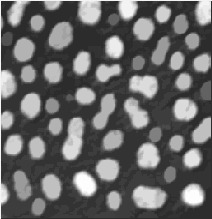
\includegraphics[width=\linewidth]{report/exam/images/immed_gray_inv_20051218_frgr4.jpg}
  \caption{Original image without operations}\label{fig:image-1}
\endminipage\hfill
\minipage{0.32\textwidth}
  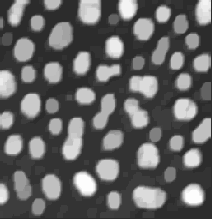
\includegraphics[width=\linewidth]{report/exam/images/exercise_05a_output-01_1.png}
  \caption{Image after applying opening once}\label{fig:awesome_image2}
\endminipage\hfill
\minipage{0.32\textwidth}%
  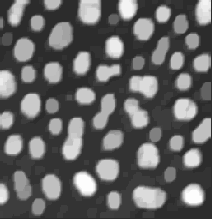
\includegraphics[width=\linewidth]{report/exam/images/exercise_05a_output-02.png}
  \caption{Image after applying opening twice}\label{fig:awesome_image3}
\endminipage
\end{figure}

\section{True or false questions.}

\begin{itemize}
    \item Indicate whether dilations ($\delta$) and erosions ($\epsilon$) are idempotent. (\textbf{FALSE})
    \item Indicate whether openings ($\gamma$) and closings ($\varphi$) are idempotent. (\textbf{TRUE}).
    \item Indicate whether alternated filters ($\varphi\gamma$ and $\gamma\varphi$) are idempotent. (\textbf{TRUE})
\end{itemize}

\section{Enumerate one segmentation algorithm based in neighbourhood processing.}

\section{Which kind of algorithms / techniques are commonly used for semantic image segmentation?}

\end{document}
